\documentclass[extendedabs]{bmvc2k}
\usepackage[ruled]{algorithm2e}
\begin{document}

\section*{digital image processing hw2}
\subsection*{problem 1: guided filter}

Guided filter \cite{guided} is an explicit image filter which have the edge-preserving 
smoothing property like the bilateral filter, but also handles gradient reversal artifacts
within O(N) time complexity. 
In guided filter, filter output is assumed to be a linear transformation of guidance $I$
with linear coefficients $a_k$, $b_k$ in a window $\omega_k$ of center pixel $k$.
Coefficients are optimized to minimize the difference between $q$ and input $p$:
\[E(a_k,b_k) = \sum_{i \in \omega_k}((a_kI_i + b_k - p_i)^2 + \epsilon a_k^2)\]
\[a_k=\frac{1/|\omega|\sum_{i \in \omega_k}I_ip_i - \mu_k\bar{p_k}}{\sigma_k^2+\epsilon}\]
\[b_k=\bar{p_k} - a_k\mu_k\]
where $\mu_k$, $\sigma_k^2$ are the mean, variance of $I$ in $\omega_k$, 
$\bar{p_k}=1/|\omega|\sum_{i \in \omega_k}p_i$. 
When applying the window in the image, several windows $\omega_k$ can affect a same pixel.
Thus output $q$ can be averaged from all the possible windows:
\[q_i = 1/|\omega|\sum(a_kI_i + b_k)\]

Since the box filters are the only filters applied in calculating the output image,
by using the integral image technique, the time complexity of guided filter becomes O(N).

\begin{figure}[h]
    \centering
    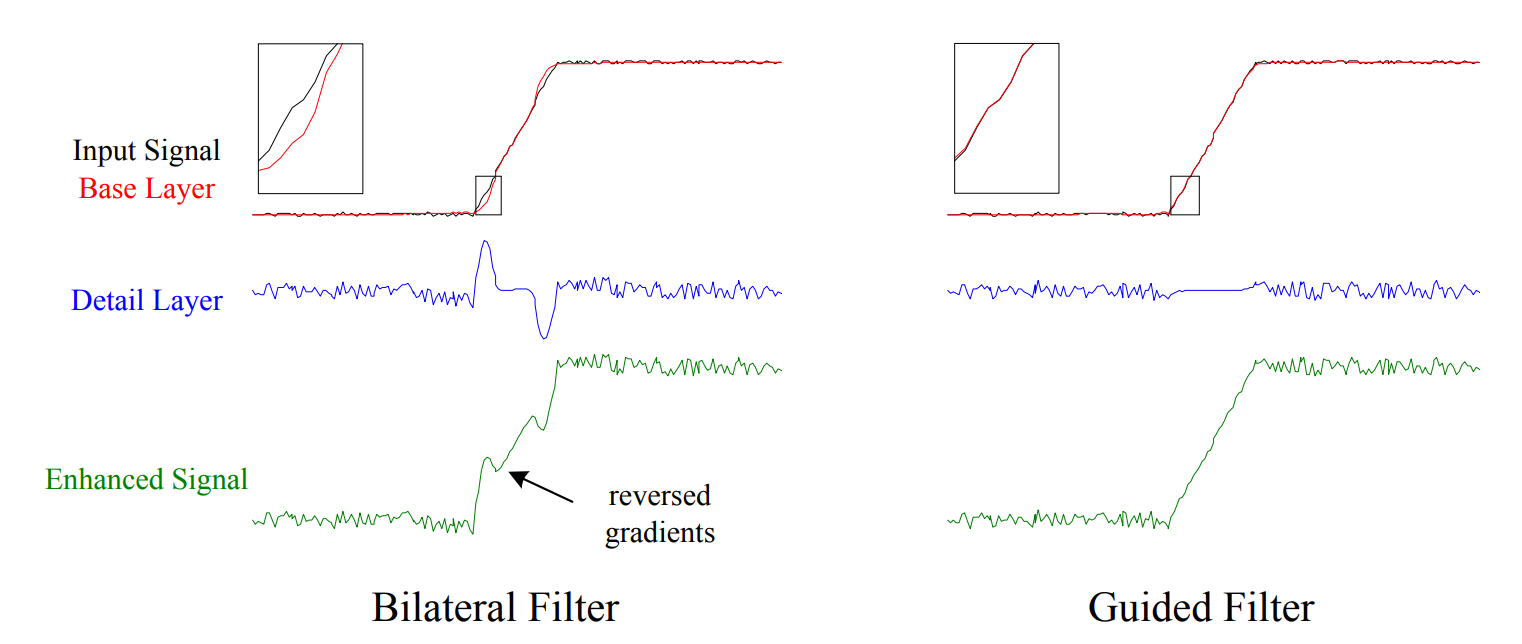
\includegraphics[width=\linewidth]{hw2_1_1}
    \caption{gradient reversal effect from bilateral filter and the corresponding guided filter result}
    \label{fig:1}
\end{figure}

Another good property of the above equation is that $\bigtriangledown q$ can be approximated
as a scaling of $\bigtriangledown I$ only when big intensiy change causes small value for
$\bigtriangledown \bar{a_i}$, $\bigtriangledown \bar{b_i}$ where
$\bar{a_i} = 1/|\omega|\sum_{k \in \omega_i}a_k$ and 
$\bar{b_i} = 1/|\omega|\sum_{k \in \omega_i}b_k$. By assuring scaling relation only on edge,
unlike bilateral filter, which gets confused when trying to smooth edge component, gets stable on
the edge and prevents gradient reversal problem.  
Visual representation of gradient preserving property in the guided filter can 
be found in \figurename{\ref{fig:1}}.

Actual result, \figurename{\ref{fig:4}}, also shows that gradient reversal effect is diminished by 
applying guided filter rather than bilateral filter.
\begin{figure}[h]
    \centering
    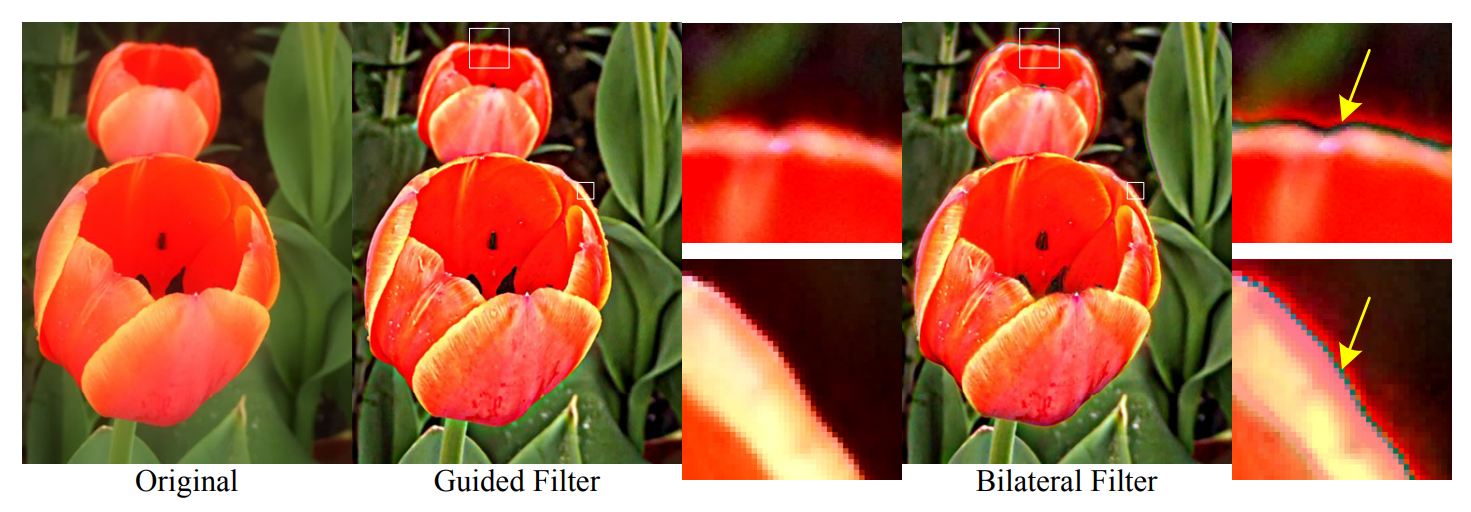
\includegraphics[width=\linewidth]{hw2_1_4}
    \caption{gradient reversal effect from bilateral filter and the corresponding guided filter result}
    \label{fig:4}
\end{figure}

From the equation above, the output can be also defined as a linear transformation of the input.
\[q_i = \sum_{j}W_ij(I)p_j\]
\[W_ij(I) = 1/|\omega|^2\sum_{k:(i,j) \in \omega_k}(1 + \frac{(I_i - \mu_k)(I_j - \mu_k)}{\sigma_k^2 + \epsilon})\]

\begin{figure}[h]
    \centering
    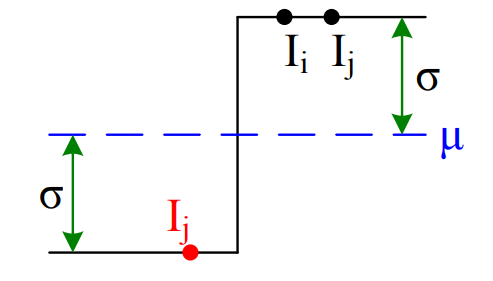
\includegraphics[width=0.3\linewidth]{hw2_1_3}
    \caption{relation between $W_ij$ and the directions of $I_i$, $I_j$}
    \label{fig:3}
\end{figure}

This form gives a good intuition about edge-preserving property of the guided filter;
As in \figurename{\ref{fig:3}}, when $I_i$ and $I_j$ are on the other side of an edge, 
then $(I_i-\mu_k)(I_j-\mu_k)$ becomes negative, 
thus $(1 + \frac{(I_i - \mu_k)(I_j - \mu_k)}{\sigma_k^2 + \epsilon})$ gets close to zero,
resulting small $W_ij$ value.
\figurename{\ref{fig:5}} contains kernel values of both guided filter and bilateral filter.
It can be also seen that as in bilateral filter, guided filter preserved edge component.

\begin{figure}[h]
    \centering
    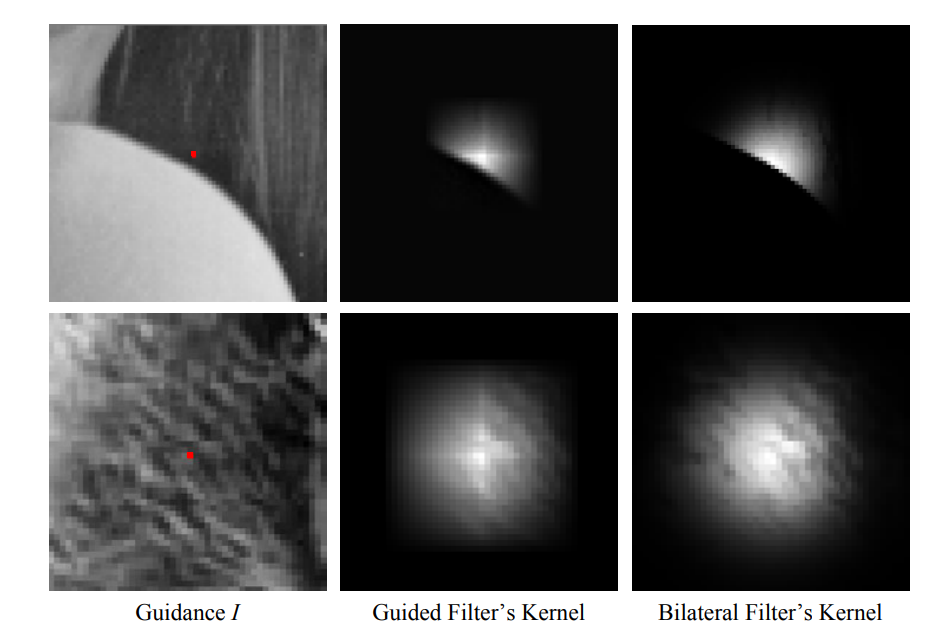
\includegraphics[width=0.8\linewidth]{hw2_1_5}
    \caption{kernel valud of guided filter/bilateral filter}
    \label{fig:5}
\end{figure}


\subsection*{problem 1: rolling guidance filter}

Rolling guidance filter \cite{rolling} is a scale-aware local operation filter that controls smoothing
details with a scale measure, by which small-scale structures can be removed while preserving others.
Rolling guidance filter consists of two steps; small structure removal and edge recovery.
At beginning, gaussian filter is used to remove small structures, which also involves blurring at
large-scale intensity variations.
\[G(p) = 1/K_p\sum_{q \in N(p)}exp(-\frac{||p-q||^2}{2\sigma_s^2})I(q)\]
\[K_p = \sum_{q \in N(p)}exp(-\frac{||p-q||^2}{2\sigma_s^2})\]
The next edge recovery step iteratively recovers edge with joint bilateral filter, with the guidance
image as its previous step output. $J^t$ stands for the recovery result from the $t$-th iteration.
\[J^{t+1}(p) = 1/K_p\sum_{q \in N(p)}exp(-\frac{||p-q||^2}{2\sigma_s^2}-\frac{||J^t(p)-J^t(q)||^2}{2\sigma_r^2})I(q)\]
\[K_p = \sum_{q \in N(p)}exp(-\frac{||p-q||^2}{2\sigma_s^2}-\frac{||J^t(p)-J^t(q)||^2}{2\sigma_r^2})\]
These two steps can be merged if $J^0$ is a constant-value image. Assign $J^t$ as a constant $C$, then
the resulting $J^t$ has the form exactly same as gaussian filter.

\begin{algorithm}
\caption{rolling guidance filter}
    $J^0 \gets$ constant image\;
    \For{$t = 1:num\_iter$}{
        $J^t \gets joint\_bilateral(I, J^{t-1}, \sigma_s, \sigma_r)$\;
    }
    return $J^{num\_iter}$\;
\end{algorithm}

It can be seen in \figurename{\ref{fig:2}} the detailed iteration process and its output.
As the iteration progresses, small structure smoothes out while large structure gets blurred
at the first phase and then the edge is recovered.
\begin{figure}[h]
    \centering
    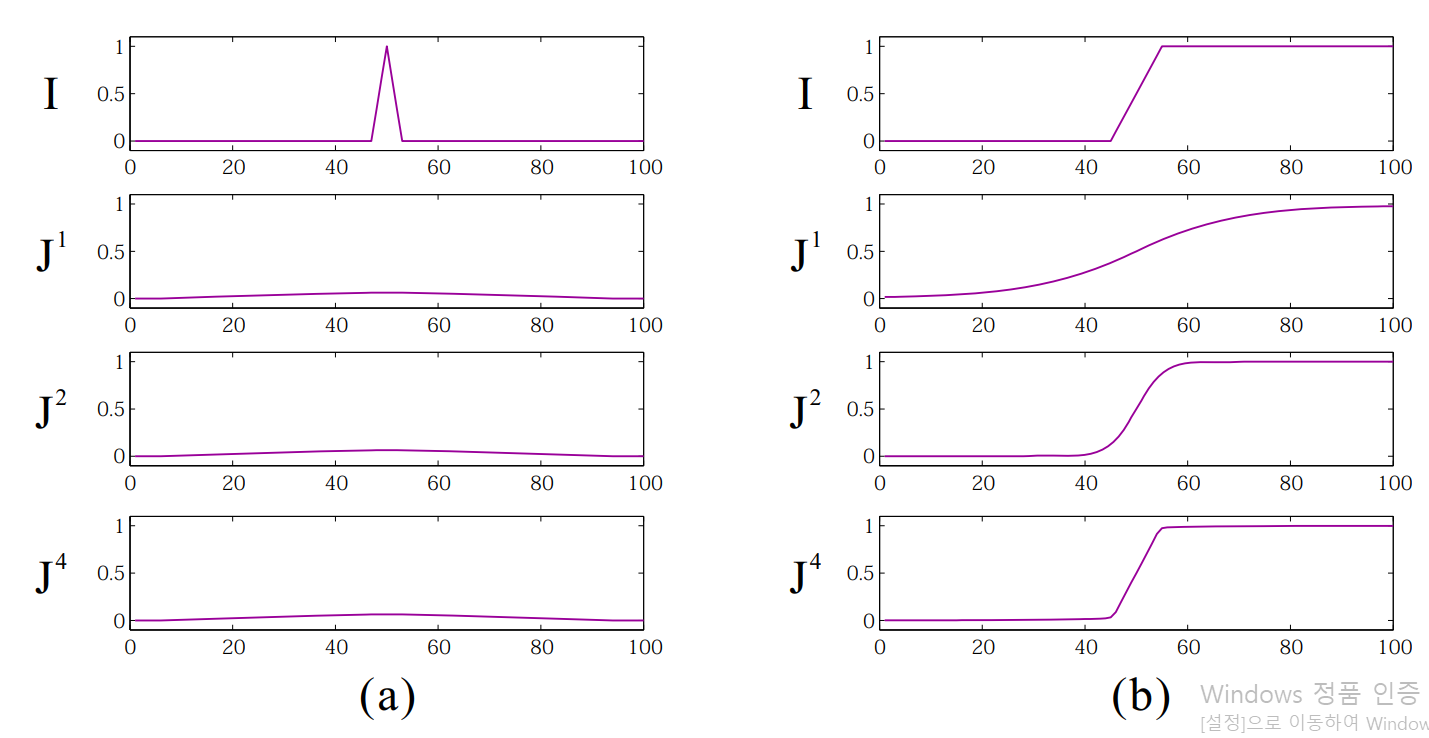
\includegraphics[width=\linewidth]{hw2_1_2}
    \caption{iteration result $J^t$ in 1-D signal. (a) small structure (b) large structure}
    \label{fig:2}
\end{figure}

\subsection*{problem 2: cross image filtering}

blah

\subsection*{problem 3: texture removal}

blah

\subsection*{problem 4: WLS filter}

blah

\subsection*{references}

\begin{thebibliography}{9}
    \bibitem{guided}
    K. He, J. Sun, and X. Tang, Guided Image Filtering, ECCV 2010.
    
    \bibitem{rolling}
    Q. Zhang et al., Rolling Guidance Filter, ECCV 2014.
\end{thebibliography}

\end{document}
